\subsubsection{Missatges d'error del SDK}

\paragraph{}
En cas que alguna operació del SDK no acabi de la forma prevista, s'ensenyarà un error indicant que el problema ha recaigut a la banda de FamilySearch i s'indicarà quin ha estat l'error retornat des de l'organització.

Un possible error, per exemple, podria ser quan alguna de les persones retornades, no pot ser trobada a l'arbre familiar. L'estil utilitzant per representar els errors de l'API és el mateix que pels errors de validació del formulari i un exemple pot ser vist en la imatge~\ref{fig:fsError}.

\begin{figure}[h]
    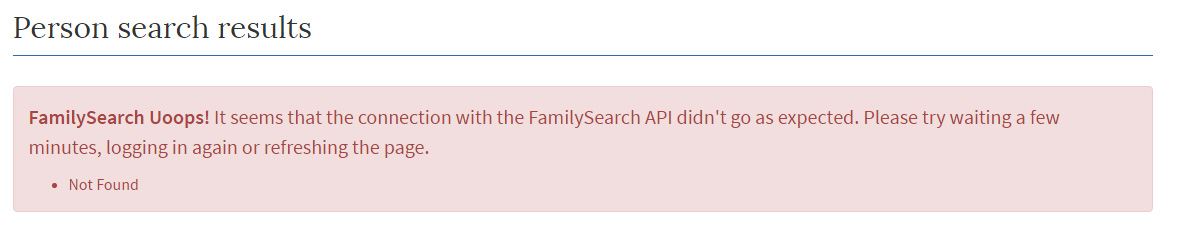
\includegraphics[width=\linewidth]{11/02_searchPersons/05_familySearchError}
    \centering
    \caption{Exemple de missatge d'error del SDK}\label{fig:fsError}
\end{figure}
